\documentclass[12pt,final,twoside]{report}
%%%%%%%%%%%%%%%%%%%%%%%%%%%%%%%%%%%%%%%%%%%%%%%%%%%%%%%%%%%%%
% Some credits:
% The template initially was created by Prof. Dr. Holger Karl/Uni Paderborn '2006
% and was expanded and updated by Dipl.-Inform. Stefan Heinrich/Uni Paderborn/Uni Hamburg since 2008.
% Suggestions for changes are always welcome.
%%%%%%%%%%%%%%%%%%%%%%%%%%%%%%%%%%%%%%%%%%%%%%%%%%%%%%%%%%%%%
% Meta information:
\newcommand{\trtitle}{Visual-Audio Integration for Object Recognition}
\newcommand{\trtype}{Master thesis} %{Diplomarbeit} %{Dissertation}
\newcommand{\trcourseofstudies}{Intelligent Adaptive Systems} %{Bioinformatik} 
\newcommand{\trauthor}{Weipeng He}
\newcommand{\trauthortitle}{} %{Dipl.-Inform.\ }
\newcommand{\tremail}{2he@informatik.uni-hamburg.de}
\newcommand{\trmatrikelnummer}{6411529}
\newcommand{\trstrasse}{Hagenbeckstra\ss e 60}
\newcommand{\trort}{22527 Hamburg}
\newcommand{\trgutachterA}{\href{mailto:zhang@informatik.uni-hamburg.de}{Prof. Dr. Jianwei Zhang}}
\newcommand{\trgutachterB}{\href{mailto:maeder@informatik.uni-hamburg.de}{Dr. Andreas M\"ader}}
%\newcommand{\trbetreuung}{\href{mailto:tbd@informatik.uni-hamburg.de}{Dipl.-Inform. To Be Defined}}
\newcommand{\trfach}{Technical Aspects of Multimodal Systems, TAMS}
\newcommand{\trdate}{30.03.2015}
\newcommand{\trkeywords}{Multimodal, HMM, Object Recognition}

%%%%%%%%%%%%%%%%%%%%%%%%%%%%%%%%%%%%%%%%%%%%%%%%%%%%%%%%%%%%%
% Languages:

% Falls die Ausarbeitung in Deutsch erfolgt:
% \usepackage[german]{babel}
% \usepackage[T1]{fontenc}
% \usepackage[latin1]{inputenc}
% \usepackage[latin9]{inputenc}                     
% \selectlanguage{german}

% If the thesis is written in English:
\usepackage[english]{babel}                         
\selectlanguage{english}

%%%%%%%%%%%%%%%%%%%%%%%%%%%%%%%%%%%%%%%%%%%%%%%%%%%%%%%%%%%%%
% Bind packages:
\usepackage{acronym}                    % Acronyms
\usepackage{algorithmic}                % Algorithms and Pseudocode
\usepackage{algorithm}                  % Algorithms and Pseudocode
\usepackage{amsfonts}                   % AMS Math Packet (Fonts)
\usepackage{amsmath}                    % AMS Math Packet
\usepackage{amssymb}                    % Additional mathematical symbols
\usepackage{amsthm}
\usepackage{booktabs}                   % Nicer tables
%\usepackage[font=small,labelfont=bf]{caption} % Numbered captions for figures
\usepackage{color}                      % Enables defining of colours via \definecolor
\definecolor{uhhRed}{RGB}{226,0,26}     % Official Uni Hamburg Red
\definecolor{uhhGrey}{RGB}{136,136,136} % Official Uni Hamburg Grey
\definecolor{uhhLightGrey}{RGB}{220, 220, 220}
\usepackage{fancybox}                   % Put equations in a frame
\usepackage{fancyhdr}                   % Packet for nicer headers
%\usepackage{fancyheadings}             % Nicer numbering of headlines
\usepackage[body={5.8in,9in}]{geometry} % Type area (size, margins...)

%\geometry{a4paper,outer=3.35cm}        % !!!Release version (Normal margins)
%\geometry{a4paper,outer=2.5cm}         % !!!Print version (Additional margin on the left for the binding)
%\geometry{a4paper}                     % !!!Proofread version (Additional margin on the right for corrections)
\geometry{a4paper,outer=3.15cm}         % !!!Draft version (Same margins on left and right)
%\geometry{paperheight=10.0in,paperwidth=6.4in,top=0.51in,left=0.3in}  % !!!Developer version (Minimal margins)

\usepackage{graphicx}                   % Inclusion of graphics
%\usepackage{latexsym}                  % Special symbols
\usepackage{longtable}                  % Allow tables over several parges
\usepackage{listings}                   % Nicer source code listings
\usepackage{multicol}                   % Content of a table over several columns
\usepackage{multirow}                   % Content of a table over several rows
\usepackage{rotating}                   % Alows to rotate text and objects
\usepackage{tabularx}                   % Tables with fixed width but variable rows
\usepackage{url,xspace,boxedminipage}   % Accurate display of URLs

%%%%%%%%%%%%%%%%%%%%%%%%%%%%%%%%%%%%%%%%%%%%%%%%%%%%%%%%%%%%%
% PDF Information und Definitions:
\author{\trauthor}

\ifx\pdftexversion\undefined
\usepackage{hyperref}
\else
\usepackage[colorlinks=false,           % link is colores (true) or has colored frame (false)
            linkcolor=uhhRed,           % case colorlinks=true: define color.
            urlcolor=uhhRed,
            citecolor=uhhRed,
            bookmarks,                  % Place bookmarks erstellen
            bookmarksopen=true,         % Bookmarks will be shown at start (true/false)
            pdfpagemode=UseOutlines,    
            bookmarksopenlevel=1,       % Define the depth of shown links
            bookmarksnumbered,          % Numbers of chapers in Bookmarks
            pdftitle={\trtitle},
            pdfsubject={\trtype},
            pdfkeywords={\trkeywords},
            pdfauthor={\trauthor},
            plainpages=false
            ]{hyperref}
\fi

\ifx\pdftexversion\undefined
\else
\pdfoutput=1                            % Disable PDF-Output
\pdfimageresolution=1200
\pdfcompresslevel=2                     % 0 = no compression, 9 = strongest compression
\fi

%%%%%%%%%%%%%%%%%%%%%%%%%%%%%%%%%%%%%%%%%%%%%%%%%%%%%%%%%%%%%
% Configurationen:

\hyphenation{whe-ther}                  % Manually use: "\-" in a word: Staats\-ver\-trag

%\lstloadlanguages{C}                   % Set the default language for listings
\DeclareGraphicsExtensions{.pdf,.jpg,.png,.eps} % first try pdf, then eps, png and jpg
\graphicspath{{./fig/}}                 % Path to a folder where all pictures are located
\pagestyle{fancy}                       % Use nicer header and footer

% Redefine the environments for floating objects:
\setcounter{topnumber}{3}
\setcounter{bottomnumber}{2}
\setcounter{totalnumber}{4}
\renewcommand{\topfraction}{0.9}        %Standard: 0.7
\renewcommand{\bottomfraction}{0.5}     %Standard: 0.3
\renewcommand{\textfraction}{0.1}       %Standard: 0.2
\renewcommand{\floatpagefraction}{0.8}  %Standard: 0.5

% Tables with a nicer padding:
\renewcommand{\arraystretch}{1.2}

% Chapter and Sections will not be written in capitals
\renewcommand{\chaptermark}[1]{\markboth{\chaptername \ \thechapter.\ #1}{}}
\renewcommand{\sectionmark}[1]{\markright{\thesection.\ #1}}

%%%%%%%%%%%%%%%%%%%%%%%%%%%%
% Additional 'theorem' and 'definition' blocks:
\theoremstyle{plain}
\newtheorem{theorem}{Theorem}[chapter]
%\newtheorem{theorem}{Satz}[chapter]    % Wenn in Deutsch geschrieben wird.
\newtheorem{axiom}{Axiom}[chapter]     
%\newtheorem{axiom}{Fakt}[chapter]      % Wenn in Deutsch geschrieben wird.
%Usage:%\begin{axiom}[optional description]%Main part%\end{fakt}

\theoremstyle{definition}
\newtheorem{definition}{Definition}[chapter]

%Additional types of axioms:
\newtheorem{lemma}[axiom]{Lemma}
\newtheorem{observation}[axiom]{Observation}

%Additional types of definitions:
\theoremstyle{remark}
%\newtheorem{remark}[definition]{Bemerkung} % Wenn in Deutsch geschrieben wird.
\newtheorem{remark}[definition]{Remark} 

%%%%%%%%%%%%%%%%%%%%%%%%%%%%
% Provides TODOs within the margin:
\newcommand{\TODO}[1]{\marginpar{\emph{\small{{\bf TODO: } #1}}}}

%%%%%%%%%%%%%%%%%%%%%%%%%%%%
% Abbreviations and mathematical symbols
\newcommand{\modd}{\text{ mod }}
\newcommand{\RS}{\mathbb{R}}
\newcommand{\NS}{\mathbb{N}}
\newcommand{\ZS}{\mathbb{Z}}
\newcommand{\dnormal}{\mathit{N}}
\newcommand{\duniform}{\mathit{U}}

\newcommand{\erdos}{Erd\H{o}s}
\newcommand{\renyi}{-R\'{e}nyi}
% it is recommented to define complex terms as expression/newcommand and use the expression in the tex instead.

%%%% added by hwp %%%%
\usepackage[labelfont=bf,width=.8\textwidth]{caption}
\usepackage{subcaption}
\usepackage[symbol*]{footmisc}
\usepackage[capitalize]{cleveref}
\newcommand{\crefrangeconjunction}{--}
\usepackage{tikz}

\newcommand{\includetexfig}[1]{\input{fig/#1.tex}}
%\newcommand{\includesvg}[1]{\def\svgwidth{.6\textwidth}\footnotesize\input{fig/#1.eps_tex}}

\DeclareMathOperator*{\argmin}{arg\,min}
\DeclareMathOperator*{\argmax}{arg\,max}
%%%% end of added by hwp %%%%

%%%%%%%%%%%%%%%%%%%%%%%%%%%%%%%%%%%%%%%%%%%%%%%%%%%%%%%%%%%%%
% Document:

\begin{document}

\pagenumbering{Roman}                   % Roman pagenumbering for lists and meta pages
\renewcommand{\headheight}{14.5pt}      % Size of headings

\thispagestyle{empty}
\fancyhead[LO,RE]{}                     % Define the header style for the meta pages

%%%%%%%%%%%%%%%%%%%%%%%%%%%%
% Cover sheet

\begin{titlepage}
%---Possibility 1:
    \begin{flushleft}
        
\includegraphics[width=85mm]{uhhLogoL.pdf}\\
    \end{flushleft}
%---Possibility 2:
%\includegraphics*[width=0.09\textwidth]{uhhIconR_}
%\parbox[c]{10cm}{
%    \begin{center}
%    Universit"at Hamburg --- MIN-Fakult"at\\
%    \trfachgruppe
%    \end{center}
%    }\hfill
%\includegraphics*[width=0.09\textwidth]{infIcon_}
%\vspace{0.2cm}
%---
    \rule{\textwidth}{0.4pt}
        \newline
        \vspace{2.0cm}
        \begin{center}
          \LARGE \textbf{\trtitle}
        \end{center}
    \vspace{2.0cm}
    \begin{center}
      \textbf{\trtype}\\
      %am Fachgebiet \trfach\\
      im Arbeitsbereich \trfach\\
      \trgutachterA\medskip\\
      Department Informatik\\
      MIN-Fakult\"at\\
      Universit\"at Hamburg \\[0.5cm]
      vorgelegt von \\
      \textbf{\trauthortitle\href{mailto:\tremail}{\trauthor}}\\
      am\\
      \trdate
    \end{center}
    \vspace{1cm}
    \begin{center}
    \begin{tabular}{ll}
    Gutachter: & \trgutachterA \\
                   & \trgutachterB \\
    %Betreuung: & \trbetreuung \\    	% Adviser are not allowed to demand getting credited, but are happy getting credited by the students initiative
    \end{tabular}
    \end{center}
    \vfill
    \begin{tabular}{l}
    \trauthor \\
    Matrikelnummer:  \trmatrikelnummer \\
    \trstrasse \\
    \trort
    \end{tabular}
    \newline
    \rule{\textwidth}{0.4pt}
    \newpage 
\end{titlepage}

    %backsite of cover sheet is empty!
\thispagestyle{empty}
\hspace{1cm}
\newpage

%%%%%%%%%%%%%%%%%%%%%%%%%%%%
% Abstract:
\section*{Abstract}\label{sec:abstract}
%\fancyhead[LE,RO]{\it Abstract}
%\addcontentsline{toc}{chapter}{\numberline{}Abstract}
Your English abstract here (mandatory if written in English and recommended otherwise).

\fancyhead[LE,RO]{\it Abstract}

\cleardoublepage

%%%%%%%%%%%%%%%%%%%%%%%%%%%%
% Lists:
\setcounter{tocdepth}{1}               % depth of the table of contents (for BSc and MSc Thesis 1 is recommented)
\fancyhead[LE,RO]{\it Contents}
\tableofcontents
\cleardoublepage
% List of Figures and List of tables are optional. -> Not needed in most theses.
\fancyhead[LE,RO]{\it List of Figures}
\listoffigures
\cleardoublepage
\fancyhead[LE,RO]{\it List of Tables}
\listoftables
\cleardoublepage
%\lstlistoflistings
%\cleardoublepage

\fancyhead[LE]{\it \leftmark}           % Define the header style for the text pages
\fancyhead[RO]{\it \rightmark}          % Define the header style for the text pages
\fancyhead[LO,RE]{}                     % Define the header style for the text pages

%%%%%%%%%%%%%%%%%%%%%%%%%%%%
% The content will be included here:
\pagenumbering{arabic}

\chapter{Introduction}
Considering how humans recognize objects, we use not only our vision, but also perceptions of other modalities, like auditory, haptic and olfactory perceptions. These extra perceptions provide complementary information. For example, a paper cup might have the same shape as a ceramic cup, and it is difficult to distinguish them only with vision. However, if we make some sound of them by knocking or touch them, we can use auditory or haptic information to tell the difference. This idea of multimodal object recognition is also applied to robotic systems.

\section{Background}

\section{Related Work}

\subsection{Multimodal pLSA Model}
Nakamura et al.~\cite{nakamura_multimodal_2007} proposed an unsupervised object categorization method for robots based on visual, audio and haptic information. They used a multimodal pLSA model, which is extended from the pLSA model described in~\cite{sivic_discovering_2005}, for the categorization.

In their experiment, a robot hand was used to grasp and shake the objects. During the interaction, visual, audio and haptic information were collected by a camera at the side, a microphone and pressure sensors on the robot finger. Afterwards, the data were processes separately as follows:
\begin{description}
  \item[Visual Information] \hfill \\
    Each image frame was represented using a bag-of-words model with scale and affine invariant salient region detector~\cite{mikolajczyk_scale_2004} and SIFT descriptor~\cite{lowe_distinctive_2004}. The visual vocabulary was generated by clustering the local descriptors in a collection of images into 600 clusters using k-means algorithm. The collection of images are 100 indoor images, which are independent of the objects in their experiment.
  \item[Audio Information] \hfill \\
    For each audio frame, a 13-dimensional MFCC feature was first calculated and then represented as a bag-of-words model with a vocabulary of 50 clusters. The vocabulary was generated with speech and noises.
  \item[Haptic Information] \hfill \\
    For each grasp of an object, a 2-dimensional feature vector was collected by the pressure sensors on the robot finger. Then, the feature vectors were vector quantized with 5 clusters, which was generated in advance.
\end{description}

They tested the unsupervised categorization on 40 objects in 8 categories. The objects were toys like stuffed toys, rattles, tambourines and balls. It was shown that their categorization result of using three modalities was identical to the categorization result of human subject. However, categorization using one modality alone did not work as well.

Furthermore, they also tested the performance of category and property inference of an unseen object. By using ``fold in'' heuristic~\cite{hofmann_probabilistic_1999}, they correctly inferred the categories of all the objects in leave-one-out cross validation. For the property inference, their method can infer the auditory and haptic properties when given only the visual cue of the object.

\subsection{Behavior-Grounded Relational Learning}
Another multimodal object categorization approach is the behavior-grounded relational learning proposed by Sinapov and Stoytchev~\cite{sinapov_object_2011}. Different from the aforementioned multimodal pLSA approach, they used different features and a supervised learning method.

They used an upper-torso humanoid robot to interact with the objects and collect proprioceptive and auditory information. The interactions included five exploratory behaviors, which are lift, shake, drop, crush and push. The proprioceptive data was recorded with 7 joint torque sensors and the auditory data was recorded by a microphone mounted on the robot head.

The method for extracting proprioceptive and auditory features were described in~\cite{bergquist_interactive_2009} and~\cite{sinapov_interactive_2009}, respectively. Since the interactions spanned over time, the data recorded were sequences of vectors. Here, a proprioceptive vector consisted of the joint torques, and a auditory vector was a Short Time Fourier Transform (STFT) of the raw audio recording. These vectors were further quantized using Self-organizing Map (SOM). Then, one modality of one behavior execution could be represented as a sequence of nominal values, that are the states in the SOM. Furthermore, the similarity between two different sequence can be calculated with Needleman-Wunch alignment algorithm~\cite{needleman_general_1970}.

Based on the similarity of executions recordings, they constructed the relational features. The relational features of an object are the average similarities to a known object sets (for example the objects which are or are not plastic cups). The sets were the objects of the 6 categories, which are plastic cups, pop cans, metal objects, soft objects, empty bottles and objects with content. And, with 10 sensorimotor context (a behavior-modality combination), a object is represented by a $10 \times 2 \times 6 = 120$ dimensional vector.

Consequently, they applied discriminative methods, like Support Vector Machine, k-Nearest Neighbor and Decision Tree, for learning the object category. They evaluated these methods with Cohen's kappa coefficient~\cite{cohen_coefficient_1960}. Their approach achieved kappa coefficient from 0.4 to .85 for the recognition.

\section{Contribution}

\section{Thesis Outline}

\cleardoublepage
\chapter{Visual Features}
\label{ch:visual}

Visual object recognition has been extensively studied in the recent decade. Vision is very essential for both humans and artificial agents to recognize an object, since the appearance of the object provides us with the most direct and informational features. Numerous features have been proposed for visual object recognition and they have been used in a variety of applications.

In this chapter, we will present the state-of-the-art representation of object images using local features and the bag-of-words model, which is based on local features.

\iffalse
\begin{figure}[tbhp]
  \centering
  \begin{subfigure}[b]{.3\textwidth}
    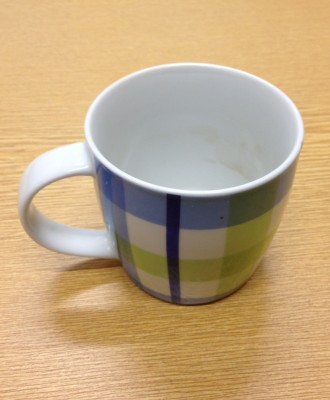
\includegraphics[width=\textwidth]{themug}
    \caption{Sam's coffee mug}
  \end{subfigure}
  ~
  \begin{subfigure}[b]{.3\textwidth}
    \centering
    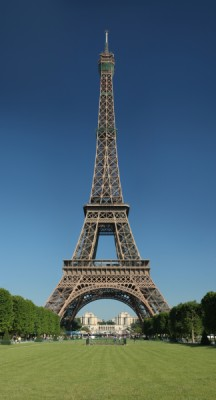
\includegraphics[width=.7\textwidth]{tour_eiffel}
    \caption{The Eiffel Tower\footnotemark}
  \end{subfigure}
  ~
  \begin{subfigure}[b]{.3\textwidth}
    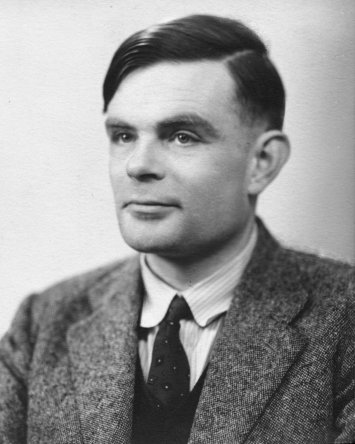
\includegraphics[width=\textwidth]{turing}
    \caption{Alan Turing}
  \end{subfigure}
  \caption{Examples of specific objects.}
  \label{fig:specific}
\end{figure}
\footnotetext{``Eiffel Tower'' by \href{http://commons.wikimedia.org/wiki/User:Benh}{Benh}. Licensed under \href{http://creativecommons.org/licenses/by-sa/3.0}{CC BY-SA 3.0}.}

Concerning object recognition, there are two types of tasks been studied: specific object recognition and object category recognition~\cite{grauman_visual_2011}. The specific object recognition is the task of recognizing a particular object, place or person. Examples of this case are Sam's coffee mug, the Eiffel tower or Alan Turing. These objects (or person) have little variation in appearance and shape. 

\begin{figure}[tbhp]
  \centering
  \begin{subfigure}[b]{.45\textwidth}
    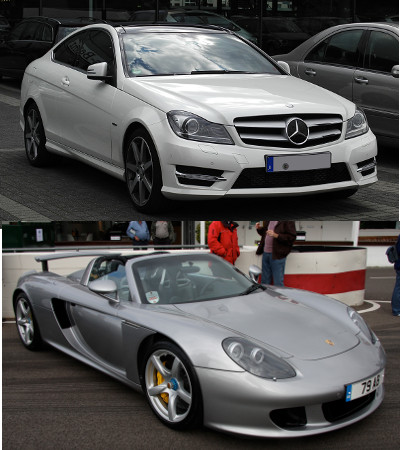
\includegraphics[width=.89\textwidth]{cars} % figure from public domain
    \caption{Cars\footnotemark}
  \end{subfigure}
  ~
  \begin{subfigure}[b]{.45\textwidth}
    \centering
    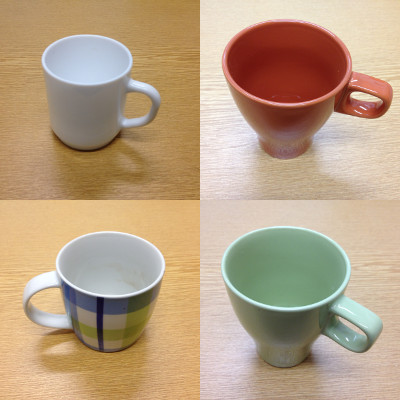
\includegraphics[width=\textwidth]{mugs}
    \caption{Coffee Mugs}
  \end{subfigure}
  \caption{Examples of generic objects categories.}
  \label{fig:generic}
\end{figure}
\footnotetext{The upper photo is ``Mercedes-Benz C 250'' by \href{http://commons.wikimedia.org/wiki/User:M_93}{M 93}. Licensed under \href{http://creativecommons.org/licenses/by-sa/3.0/de}{CC BY-SA 3.0 de}.
The lower photo is ``Porsche Carrera GT'' by \href{http://www.flickr.com/people/32659528@N00}{Brian Snelson}. Licensed under \href{http://creativecommons.org/licenses/by/2.0}{CC BY 2.0}}

Unlike the specific case, generic object category recognition deal with classifying an instance to a category, for example, telling a object is an instance of cars or coffee mugs. In this case, the objects belongs to the same category have the same conceptual meaning, but may vary in appearance and shape.

Different features are designed for the two tasks. In this chapter, we will present the basic concepts of local features and the SIFT descriptor as an example of local features. We will also introduce the bag of visual words model, which is a good solution to generic object category recognition.
\fi

%A category can also be a function or an attribute of the object, like objects that can be sit on or soft objects.

%As we have seen, these two types of tasks try to solve different problems. Therefore, different features and learning methods are required. Some of the approaches will be discussed in the rest of this section.

\section{Local Features}
Thinking of representing an object in an image, one method is extracting patterns that describe the whole picture, such as using the intensities of pixels. These methods are the global image representations. However, since the structures of most object appearances are very complex and the images are also subject to lighting variations, scaling, rotations, translations as well as occlusions, such global image representations can hardly generate robust results. 

In contrast to global representations, the local feature representation uses features of a local patches or regions to describe the image. These representations are designed to be invariant to a range of image transformations, such as scaling, rotation, translation and affine deformation. The development of such local features in the past decade has made it possible to implement robust and efficient object recognition applications.

A local feature extraction consists of the following two steps: 
\begin{description}
  \item[Keypoint detection] Detect a set of points of interest (i.e. keypoints) and the region around it, in a scale- or affine-invariant manner. Examples of keypoints detection methods include the Laplacian-of-Gaussian (LoG) detector~\cite{lindeberg_feature_1998}, the difference-of-Gaussian (DoG) detector~\cite{lowe_object_1999}, Harris affine detector~\cite{mikolajczyk_scale_2004} and maximally stable external regions (MSER)~\cite{matas_robust_2004}. 
  \item[Feature description] For each keypoint, compute its descriptor, which is a feature vector that describe the local region. Examples of feature description methods include the scale invariant feature transform (SIFT) and ``speed-up'' robust features (SURF)~\cite{bay_speeded-up_2008}.
\end{description}

Once descriptors are extracted, the similarity between images can be computed via comparing the local features they have. This yields a direct application for specific object recognition.

In the following section, we will introduce the DoG detector and the SIFT descriptor, as these methods are used in our system.

\subsection{The difference-of-Gaussian Detector}
The keypoint detection should be in a way that it can be repeated with different images of the same object. Therefore, the detectors are required to be scale or affine invariant. The difference-of-Gaussian (DoG) detector is an instance of scale invariant detectors.

Given an image $I(x)$, the DoG detector finds the position $x$ and the scale $\sigma$ that maximize (locally) the difference-of-Gaussian:
\begin{equation}
  D(x,\sigma) = (G(x,k\sigma) - G(x,\sigma)) * I(x)
\end{equation}
where $G(x,\sigma)$ is the Gaussian convolution mask, $k$ is a constant and $*$ is convolution. An efficient way to calculating the DoG is first smoothing (convoluting) the image with Gaussian mask at different scale, and then subtracting the results with the adjacent scales. Local maxima are located in several layers of DoG filtered images (each at different scales), such that $D(x,\sigma)$ is larger than the eight neighbors in same layer and the nine neighbors on each of the adjacent layers.

After the local maxima are found, an additional filtering step is added, in order to remove the points on edges. This is accomplished by evaluating the Hessian matrix at the points.

At the end, the selected points with the regions surrounding them (typically, $r = 3\sigma$) are extracted for further processing.

\subsection{The SIFT Descriptor}
The scale invariant feature transform (SIFT) descriptor is one of the state-of-the-art features that are used for visual object recognition. SIFT was originally published in papers by Lowe~\cite{lowe_object_1999,lowe_distinctive_2004}. 
Although in the original papers, the SIFT descriptor is designed with the DoG detector, it can also be combined with other detection methods~\cite{mikolajczyk_performance_2005}.

Once keypoints are located, the feature description of the keypoints should be in the way that it is invariant to many image transformations. What the keypoints detectors, such as DoG detector, has already achieved is scale and translation invariance. In addition to that, the SIFT descriptor provides features that are invariant to rotation and illumination variation.

The SIFT descriptor describes a keypoint as histograms of gradient orientations. Specifically, it is computed via the following steps:
\begin{enumerate}
  \item Normalize the size and orientation of the region around the keypoint according the scale, which is the result of scale invariant detector, and the dominant orientation.
  \item The region is divided to a $16 \times 16$ regular grid. For each location, the gradient orientation is computed.
  \item These locations are again divide into a $4 \times 4$ regular grid. For each cell, the gradient orientation histogram with 8 orientation bins is computed according to the gradient magnitudes applied with a Gaussian window.
  \item Combining the $16$ histograms will result in a $16 \times 8 = 128$ dimensional vector. Normalize this vector and the result is the SIFT descriptor.
\end{enumerate}

The rotation invariance is achieved by the selecting the dominant orientation in the first step and the illumination invariance is achieved by the normalization in the last step.

\section{The Bag-of-Words Model}
While specific object recognition can be solved as matching of local features, the local feature representation cannot be directly applied to object category recognition. Local features are adequate in characterizing an exact part of a particular object. However, different objects in the same category are not identical in appearance. Thus, in this case, a valid representations should capture the common characteristics of different instances in the same class. One of the solution is the bag-of-words model~\cite{csurka_visual_2004}.

The bag-of-words model is first used in nature language processing. Its idea is considering a document as a multiset consisting of words, namely counting the number of occurrences and disregarding the sequence or position of the words. Therefore, a document can be represented as a histogram of distinctive words. The bag-of-words model has been successfully applied to a number of nature language processing and information retrieval tasks, such as text classification.

Analogous to natural text, an image, which contains a collection of keypoints (or local feature descriptors), can also regarded as an document. And, this is the idea of the bag-of-words model for computer vision. In this case, the model is also referred as bag of visual words, bag of feature or bag of keypoints. 

However, there is an essential difference between a word and a local feature descriptor, which is that a word is a nominal value while a descriptor is a real vector. Thus, a vector quantization step is carried out to map a descriptor to a visual ``word''. In most of the applications, the descriptors are quantized by matching to the nearest neighbor in a vocabulary, which is constructed in advance by clustering, such as k-means. Another benefit from quantization is that the different but similar descriptors are put into the same class. Therefore, the representation is more robust to variations between objects in the same category.

Similar to that in nature language processing, images represented by bag-of-words model can be used for further learning. These applications includes supervised classification using support vector machine or na\"ive Bayes~\cite{csurka_visual_2004} and unsupervised categorization using probabilistic latent semantic analysis or latent Dirichlet allocation~\cite{sivic_discovering_2005}.

\section{Summary}
In this chapter, we have presented the local features and the bag-of-words model for visual object recognition. The key points include:
\begin{itemize}
  \item The local feature representation is one of the state-of-art technique for computer vision. The representation is computed via keypoint detection and feature description. The results are a number of descriptors of the points of interest in the image. 
  \item The DoG detector is invariant to scaling.
  \item The SIFT descriptors are invariant to rotation and illumination variation.
  \item The Bag-of-words model, which is based on local features, is a more general representation of a image. 
\end{itemize}

\cleardoublepage
\chapter{Audio Features}
Audio signal processing has been one of the most important fields of digital signal processing. Many different audio features have been proposed to represent the audio signal. As for any system, how the data is represented affects the performance of the system dramatically. And, so is for our system. In terms of good audio features, we want to find features such that, similar sounds that human perceive also appear similar (closer) in the feature space and the number of dimensions of the feature space should be small so that it can be applied to the subsequent learning algorithms. In other words, the feature should be simple and corresponds to human perception.

Although audio features for object recognition have not been systematically studied, there has been extensive studies on audio features for speech recognition. The mel-frequency cepstrum coefficients (MFCCs) is one of the most commonly used audio features in speech recognition. Therefore, we choose MFCCs as the audio feature in our system.

In this chapter, we will present the basics about preprocessing of audio signal, namely short time Fourier transform, and the properties of the MFCCs.

\section{Short Time Fourier Transform}
The raw audio data are represented as the altitudes of the pressure changing over time, i.e. time-domain signal. However, the time-domain signal does not contain direct information of how the signal sounds like. Thus, it is difficult be analyzed. By applying the Fourier transform, we can change the signal to frequency domain. In the frequency domain, further analysis of the signal can be applied.

The power spectrum, i.e. the squared magnitude of the Fourier transform, shows how the energy is distributed in different frequency bin, but it does not show how the signal varies over time. That means it cannot specify the local information at a certain time. The solution to this problem is the short time Fourier transform (STFT), which transform the signal to the time-frequency domain.

The idea of STFT is that by using a sliding window, the signal at a short time is taken, and then applying the Fourier transform. More specifically, the STFT is defined as follows:
\begin{equation}
  X(n, k) = \sum_{m = -\infty}^{\infty} x[m]w[m-n]e^{-j \frac{2\pi k}{N} m}
\end{equation}
where $x$ is the signal, $w$ is the window function, $n$ is the index of time, $k$ is the index of frequency bin, and $N$ is the number of frequency bins. 

Common window functions include the Hann window (\cref{fig:hann}):
\begin{equation} w(n) = 0.5 (1 - \cos(\frac{2\pi n}{N-1})) \end{equation}
and the Hamming window (\cref{fig:hamming}):
\begin{equation} w(n) = \alpha - \beta \cos(\frac{2\pi n}{N-1}) \end{equation}
where $\alpha = 0.54, \beta = 1 - \alpha = 0.46$ and $N$ is the window size.
Since, most applications in practice use the fast Fourier transform to compute the STFT, the window size is selected to be an exponential of 2.

\begin{figure}[t]
  \centering
  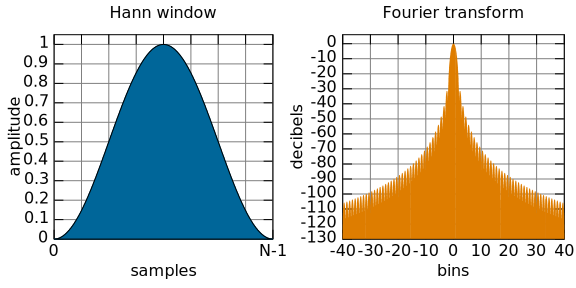
\includegraphics[width=.6\textwidth]{hann}
  \caption{Hann window.}
  \label{fig:hann}
\end{figure}

\begin{figure}[t]
  \centering
  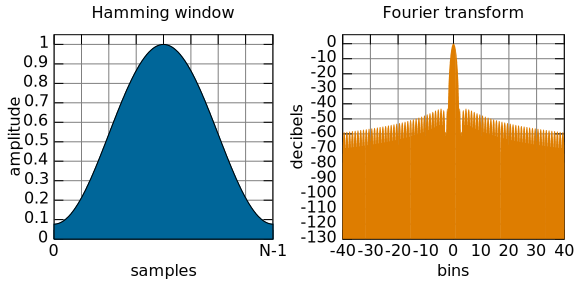
\includegraphics[width=.6\textwidth]{hamming}
  \caption{Hamming window.}
  \label{fig:hamming}
\end{figure}

The squared magnitude of the STFT yields the spectrogram:
\[ \text{Spectrogram}(n, k) = \left|X(n,k)\right|^2 \]
From the spectrogram we can clearly visualize the different frequency components of a sound and its variation over time.

Note that because the time-domain signal is real, at any time, the result of the DFT has the following properties:
\begin{itemize}
  \item $X(n,0)$ and $X[n, \frac{N}{2}]$ are real;
  \item $X(n,k) = X^*(n,N-k), k \neq 0, \frac{N}{2}$, here $^*$ is the complex conjugate.
\end{itemize}

Therefore, only the first half (index from $0$ to $\frac{N}{2}$) of the DFT contains information, while the other half is redundant. From theories of Fourier analysis, we know that the $k$th frequency bin represents the component at frequency $\frac{kf_s}{N}$, with $f_s$ being the sampling rate. The component with the highest frequency is the bin with index $\frac{N}{2}$ and its frequency is $\frac{N}{2} \times \frac{f_s}{N} = \frac{f_s}{2}$. This is, in fact, the Nyquist frequency.

\begin{figure}[t]
  \centering
  \begin{subfigure}[b]{.8\textwidth}
    \includetexfig{spec1024}
    \caption{$N=1024$}
    \label{fig:spec1024}
  \end{subfigure}

  \begin{subfigure}[b]{.8\textwidth}
    \includetexfig{spec256}
    \caption{$N=256$}
    \label{fig:spec256}
  \end{subfigure}

  \begin{subfigure}[b]{.8\textwidth}
    \includetexfig{spec64}
    \caption{$N=64$}
    \label{fig:spec64}
  \end{subfigure}

  \caption[Spectrograms with different window sizes]{Spectrograms of audio ``Hello World'' with different window sizes ($N$). (a) When the window size is $1024$, the spectrogram shows high frequency resolution, yet low time resolution.
(b) When the window size is $256$, the spectrogram shows moderate frequency resolution and time resolution.
(c) When the window size is $64$, the spectrogram shows low frequency resolution and high time resolution.
  The STFT is calculated with a shift size of half window size. }
  \label{fig:spec}
\end{figure}

One shortcoming for STFT is that the frequency resolution and time resolution is mutually limited. This limit is known as the Gabor limit. The difference of two consecutive frequency bin is $\frac{f_s}{N}$. And, one STFT is a DFT of a neighborhood of $N$ samples, i.e. $N \times \frac{1}{f_s}$ time interval. That means the time resolution is $\frac{N}{f_s}$. Therefore, the product of the two resolutions, $\frac{f_s}{N} \times \frac{N}{f_s} = 1$, is constant. 

Selecting the windows size involves trade-off between the frequency resolution and time resolution. With large window size, we can have good frequency resolution, while it can be difficult to catch the change in a short time. Vice versa, with a small windows size, we can have high time resolution. However, the frequency resolution would be low. \Cref{fig:spec} illustrates these difference.

\section{Mel-frequency Cepstrum Coefficients}
Despite the fact that the STFT gives information how the audio signal distributed at different frequencies over time, the frequency (i.e. pitch) is not the only characteristic human hear from a sound. Thus, the STFT itself is not a desired feature. However, the spectral information derived from the STFT can be further analyzed, which results in several spectral features. Among these features, the mel-frequency cepstrum coefficients (MFCCs) are commonly used for speech recognition.
The MFCCs are the coefficients of a cepstrum with frequency bands on the mel scale.

The mel scale is the scale of frequencies based on human perception of the distance in pitches. Classic study shows that human perceive the pitches in a non-linear scale~\cite{stevens_scale_1937}, which if usually formulated as~\cite{oshaughnessy_speech_1987}
\begin{equation}
  \text{mel} = 1127 \log (1 + \frac{f}{700})
\end{equation}

A cepstrum is a ``spectrum'' of log spectrum. The term cepstrum is a result of reversing the first four letters in spectrum. The idea of using a ``spectrum'' of log spectrum was prompted by detecting echo in signals~\cite{oppenheim_frequency_2004}. Consider a signal with a simple echo
\begin{equation}
  x(t) = s(t) + \alpha s(t - \tau),
\end{equation}
where $s(t)$ is the original signal and $\tau$ is the echo delay, the spectrum of the signal is
\begin{equation}
  \left| X(f) \right|^2 = \left| S(f) \right|^2 (1 + \alpha^2 + 2 \alpha \cos(2 \pi f \tau)),
\end{equation}
and the log spectrum is
\begin{equation}
  C(f) = \log \left| X(f) \right|^2 = \log \left| S(f) \right|^2 + \log (1 + \alpha^2 + 2 \alpha \cos(2 \pi f \tau)).
\end{equation}
Consider $C(f)$ as a signal of $f$, it has an additive periodic component due to the present of the $\cos$ term and its ``fundamental frequency'' is the echo delay $\tau$. Therefore, taking the Fourier transform of $C(f)$, the ``spectrum'' shows a peak at the ``fundamental frequency''. 

The computation of MFCCs consists of the following steps:
\begin{enumerate}
  \item Compute the STFT of the original time-domain signal.
  \item For each time frame, map the spectrum onto mel scale, using triangular overlapping windows.
  \item Take the log of spectrum based on mel scale.
  \item Take the discrete cosine transform of the log spectrum.
\end{enumerate}

\section{Summary}
In this chapter, we have presented some of the features for audio processing. The key points include:
\begin{itemize}
  \item The STFT is one of the basic preprocessing of audio signal, which transform time-domain signals to the time-frequency domain.
  \item The MFCC is a audio feature that gives interpretation of sounds that is similar to human perception. It also captures information such as echo in the signal.
\end{itemize}

\cleardoublepage
\chapter{Theories of Hidden Markov Model}
The hidden Markov models (HMM) are statistical models for time series data, which have been well-known and widely used by researchers~\cite{rabiner_tutorial_1989, rabiner_fundamentals_1993}. Theories of HMM are initially published by Baum and his colleagues~\cite{baum_statistical_1966, baum_maximization_1970}. They have been successfully applied to a number of research fields, including speech processing~\cite{baker_dragon_1975, rabiner_fundamentals_1993}, image processing~\cite{chen_off-line_1994}, gesture recognition~\cite{mitra_gesture_2007}, bioinformatics~\cite{koski_hidden_2001}, finance~\cite{bhar_hidden_2004}, etc.

In this chapter, we will first introduce the formal definition of the HMM and then present the algorithms for evaluating probability and estimating the model parameters.

\section{Definition of HMM} \label{sec:hmm}
A hidden Markov model describes a probability distribution of a stationary discrete-time stochastic process under certain assumptions. These assumptions include that there is an unobserved or hidden state associated with every observation at each time and the states transition meets the Markov property (i.e. Markov assumption). More precisely, for one observed sequence, $\mathbf{x}=(x_t, t \in \mathbb{N})$, and its associated state sequence, $\mathbf{q}=(q_t, t \in \mathbb{N})$, the following properties hold:

\begin{enumerate}
  \item The conditional distribution of present observation (at a certain time $t$) depends only upon the present hidden state:
  \begin{equation}
    P(x_t|q_1, \dots, q_t, x_1, \dots, x_{t-1},x_{t+1},\dots,x_T) = P(x_t|q_t), \quad t \in \mathbb{N} 
    \label{eq:ob_prob}
  \end{equation}
  \item (Markov property) The conditional probability distribution of future hidden state of the process depends only upon the present state:
  \begin{equation}
    P(q_{t+1}|q_1, \dots, q_t, x_1, \dots, x_t) = P(q_{t+1}|q_t),\quad t \in \mathbb{N}
    \label{eq:markov_prop}
  \end{equation}
\end{enumerate}

\begin{figure}[t]
  \centering
  \includetexfig{hmm}
  \caption[HMM as a Bayesian network.]{HMM as a Bayesian network. The directed edges indicate conditional dependencies. Each state variable is only conditional dependent of its previous state and each observation is only conditional dependent of the state at that time.}
  \label{fig:hmm}
\end{figure}

These conditional dependencies can be shown as a Bayesian network by unfolding the variables over time (see \cref{fig:hmm}).

Here, the observation can be on a discrete space ($x_t \in \{v_1, v_2, \dots, v_K\}$) or a continuous space ($x_t \in \mathbb{R}^d$) and the state space is discrete ($q_t \in \{1, 2, \dots, N\}$, with $N$ being the number of states). Since our system is exclusively used on continuous data, for simplicity, we will only consider the continuous observation space. Gaussian mixture models (GMM) are usually used to describe such observation probability distribution. In this case, the model is called HMM-GMM.

Given the aforementioned assumptions, one HMM can be specified with the following parameters:
\[ \lambda = (A, B, \pi) \]
such that
\begin{itemize}
  \item $A$ is the transition probability, $A = \{a_{ij}\}$, in which 
    \[ a_{ij} = P(q_{t+1} = j | q_t = i), \quad i,j \in \{1, \dots, N\} \]
  \item $B$ is the observation probability distribution, $B = \{b_j(x)\}$, in which
    \[ b_j(x) = P(x_t = x | q_t = j), \quad i,j \in \{1, \dots, N\} \]
  \item $\pi$ is the initial state distribution, $\pi = \{\pi_j\}$, in which
    \[ \pi_j = P(q_1 = j), \quad i,j \in \{1, \dots, N\} \]
\end{itemize}

As for HMM-GMM, each $b_j(x)$, more specifically, is a probability density function (pdf) of a GMM, namely
\[ b_j(x) = \sum_{k=1}^M c_{jk} \mathcal{N}(x, \mu_{jk}, \Sigma_{jk}) \]
where $c_{jk}$ is the mixture weight (coefficient), $\mu_{jk}$ is the mean and $\Sigma_{jk}$ is the covariance matrix, each of the $k$-th component in state $j$ and $\mathcal{N}$ is the pdf of the Gaussian distribution. 

With the formal definition of HMM, there are still three problems of interest to be solved, in order to use HMM for real-world applications. These problems are:
\begin{enumerate}
  \item Given a model $\lambda=(A, B, \pi)$, and an observation sequence $\mathbf{x} = (x_1 x_2 \dots x_T)$, what is the probability of the model generating such sequence, namely $P(\mathbf{x}|\lambda)$?
  \item Given a model $\lambda$, and an observation sequence $\mathbf{x}$, what is the most likely hidden state sequence $\mathbf{q} = (q_1 q_2 \dots q_t)$, namely $\argmax_{\mathbf{q}}P(\mathbf{x}|\mathbf{q},\lambda)$?
  \item Given an observation sequence $\mathbf{x}$ (or a set of observations $\{\mathbf{x}^{(i)}\}$), how do we estimate the parameters that maximize $P(\mathbf{x}|\lambda)$ (or $\prod_{i} P(\mathbf{x}^{(i)}|\lambda) $)?
\end{enumerate}

In the following section, we will show that the first and third problem can be solved using the forward/backward procedure and the Baum-Welch algorithm, respectively. The second problem can be solved using the Viterbi algorithm~\cite{forney_viterbi_1973}. However, the second problem is not related to our system, so it will not be addressed.

\section{Probability Evaluation}
Given a model $\lambda=(A, B, \pi)$, and an observation sequence $\mathbf{x} = (x_1 x_2 \dots x_T)$, we wish to calculate the probability, $P(\mathbf{x}|\lambda)$. A na\"ive solution to this is enumerating all possible state sequences and applying law of total probability, that is
\begin{equation}
  P(\mathbf{x}|\lambda) = \sum_{\text{all } \mathbf{q}} P(\mathbf{x}|\mathbf{q},\lambda) P(\mathbf{q}|\lambda) .
\end{equation}

For a fixed state sequence $\mathbf{q} = (q_1 q_2 \dots q_T)$, we can derive that
\begin{align}
  P(\mathbf{x}|\mathbf{q},\lambda) &= P(x_1|q_1,\lambda) P(x_2|q_1,q_2,x_1,\lambda) \dots P(x_T|q_1,\dots,q_T,x_1,\dots,x_{T-1},\lambda) \notag\\
  &= P(x_1|q_1, \lambda) P(x_1|q_1, \lambda) \dots P(x_T|q_T, \lambda) \notag\\
  &= b_{q_1}(x_1) b_{q_2}(x_2) \dots b_{q_T}(x_T)
\end{align}
and its probability is
\begin{align}
  P(\mathbf{q}|\lambda) &= P(q_1|\lambda) P(q_2|q_1,\lambda) P(q_3|q_1,q_2,\lambda) \dots P(q_T|q_1,\dots,q_{T-1},\lambda) \notag\\
  &= P(q_1|\lambda) P(q_2|q_1,\lambda) P(q_3|q_2,\lambda) \dots P(q_T|q_{T-1},\lambda)  \notag\\
  &= \pi_{q_1} a_{q_1q_2} \dots a_{q_{T-1}q_T} .
\end{align}
Thus we get 
\begin{equation}
  P(\mathbf{x}|\lambda) = \sum_{q_1,q_2,\dots,q_T} \pi_{q_1} b_{q_1}(x_1) a_{q_1q_2} b_{q_2}(x_2) \dots a_{q_{T-1}q_T} b_{a_T}(x_T) .
  \label{eq:prob_brute}
\end{equation}

This is a direct solution, however, the number of possible state sequences is too large, which is $N^T$. Thus, the time efficiency would be $\Theta(T N^T)$ using big theta notation. That makes it impossible to calculate when $T$ is large, which is often the case. In the following part, we will present the forward procedure and the backward procedure, which are more efficient.

\subsection{The Forward Procedure}
One of the efficient solution is using the forward procedure. Consider the forward variable, $\alpha_t(i)$, which is the joint probability or the first $t$ observations and the state at time $t$, or defined as
\begin{equation}
  \alpha_t(i) = P(x_1,\dots,x_t,q_t=i|\lambda) 
\end{equation}
it has the following properties:
\begin{enumerate}
  \item At initial time,
    \begin{equation}
      \alpha_1(i) = P(x_1,q_1=i|\lambda) = \pi_i b_i(x_1), \qquad i \in \{1,\dots,N\} .
    \end{equation}
  \item The forward variable at $t \geq 2$ can be calculated via considering it is transitioned from all the possible previous states:
    \begin{align}
      \alpha_{t+1}(j) &= P(x_1,\dots,x_{t+1},q_{t+1}=j|\lambda) \notag\\
      &= \sum_{i=1}^{N} P(x_1,\dots,x_{t+1},q_t=i,q_{t+1}=j|\lambda) \notag\\
      &= \sum_{i=1}^{N} P(x_1,\dots,x_t,q_t=i|\lambda) P(q_{t+1}=j|q_t=i,\lambda) P(x_{t+1}|q_{t+1}=j,\lambda) \notag\\
      &= \left[ \sum_{i=1}^{N} a_{ij} \alpha_t(i) \right] b_j(x_{t+1}), \qquad t \in \{1,\dots,T - 1\}, j \in \{1,\dots,N\} .
    \end{align}
  \item Take the sum of all the forward variables at time $t = T$, we get the desired calculation of the probability,
    \begin{equation}
      P(\mathbf{x}|\lambda) = \sum_{i=1}^N P(\mathbf{x},q_T=i|\lambda) = \sum_{i=1}^N \alpha_T(i) .
    \end{equation}
\end{enumerate}

By using the three properties, we can iteratively calculate all the $N$ forward variables from time $1$ to $T$. The time efficiency of the forward procedure is $\Theta(TN^2)$, which much faster than using the na\"ive solution (\cref{eq:prob_brute}).

\subsection{The Backward Procedure}
The backward procedure is an alternative solution to calculating the probability. Similar to the forward procedure, the backward procedure use the same idea of iterative calculation of variables based on previous steps, while the direction of iteration is backward, namely from $T$ to $1$. The backward variable is defined as
\begin{equation}
  \beta_t(i) = P(x_{t+1},\dots,x_T|q_t=i,\lambda) .
\end{equation}

The following properties hold:
\begin{enumerate}
  \item At time $t = T$,
    \begin{equation}
      \beta_T(i) = 1, \qquad i \in \{1,\dots,N\} .
    \end{equation}
  \item The backward variable at $t \leq T - 1$ can be calculate inductively:
    \begin{align}
      \beta_i(t) &= \sum_{j=1}^{N} P(x_{t+1},\dots,x_T,q_{t+1}=j|q_t=i,\lambda) \notag\\
      &= \sum_{j=1}^{N} P(q_{t+1}=j|q_t=i,\lambda) P(x_{t+1}|q_{t+1}=j,\lambda) P(x_{t+2},\dots,x_T|q_{t+1}=j,\lambda) \notag\\
      &= \sum_{j=1}^{N} a_{ij} b_j(x_{t+1}) \beta_{t+1}(j) , \qquad t \in \{1,\dots,T - 1\}, j \in \{1,\dots,N\} .
    \end{align}
  \item The probability is
    \begin{equation}
      P(\mathbf{x}|\lambda) = \sum_{i=1}^N P(\mathbf{x}|q_1=i,\lambda) p(q_1=i|\lambda) = \sum_{i=1}^N \beta_1(i) \pi_i .
    \end{equation}
\end{enumerate}

Same as the forward procedure, the time efficiency of the backward procedure is $\Theta(TN^2)$.

\section{Parameter Estimation}
Parameter estimation of a statistical model is the adjustment of the parameters such that the model can best match the observed or empirical data. It plays a crucial role in systems. As for HMM, we are interested in knowing what are the parameters that maximize the probability of the observation (i.e. maximum likelihood estimates):
\begin{equation}
  \lambda^* = \argmax_{\lambda} P(\mathbf{x}|\lambda) .
\end{equation}

Unlike simple models, such as Gaussian distributions, the parameters of which can be calculated directly, HMM depends on unobserved latent variables (i.e. hidden states), which make it difficult to estimate. One general solution for parameter estimation of models with latent variables is the expectation-maximization (EM) algorithm. The application of the EM algorithm for HMM is known as the Baum-Welch algorithm. We will shows these two algorithms in the following part.

\subsection{Expectation-maximization Algorithm}
The expectation-maximization algorithm is a method for finding the maximum likelihood estimates (MLE) of parameters of models with latent variables~\cite{dempster_maximum_1977}. Its idea is reestimating parameters via an expectation step (E-step) and a maximization step (M-step), in which the reestimated parameters have greater likelihood, and repeating such procedure until the likelihood reaches a maximum.

More specifically, consider observed data $\mathbf{x}$, unobserved data (i.e. latent variables) $\mathbf{z}$ and a set of parameters $\lambda$, the likelihood function is
\begin{equation}
  L(\lambda;\mathbf{x}) = P(\mathbf{x}|\lambda) = \sum_{\mathbf{z}} P(\mathbf{x},\mathbf{z}|\lambda) .
\end{equation}
The goal is maximizing the likelihood function:
\begin{equation}
  \lambda^* = \argmax_\lambda L(\lambda;\mathbf{x}).
\end{equation}

We introduce a function $Q(\lambda|\lambda')$, which is the conditional expectation of the log likelihood function with respect to the conditional distribution of $\mathbf{z}$ given $\mathbf{x}$ and $\lambda'$:
\begin{equation}
  Q(\lambda|\lambda') = \text{E}_{\mathbf{z}|\mathbf{x},\lambda'} \log P(\mathbf{x},\mathbf{z}|\lambda) .
\end{equation}

A procedure of parameters reestimation consists of the following two steps:
\begin{description}
  \item[E-Step] Compute $Q(\lambda|\lambda^{(p)})$;
  \item[M-Step] Choose $\lambda^{(p+1)}$ to be the value of $\lambda$ that maximize $Q(\lambda|\lambda^{(p)})$.
\end{description}

After each procedure it is assured that $L(\lambda^{(p+1)};\mathbf{x}) \geq L(\lambda^{(p)};\mathbf{x})$. Therefore, if we start from an initial estimate $\lambda^{(0)}$ and iteratively compute $\lambda^{(1)},\lambda^{(2)},\lambda^{(3)},\dots$, we will get a sequence of estimates, which converges to a local maximum.

The increase of likelihood function can be proved as follows: for any $\mathbf{z}$, we have
\begin{equation}
  \log P(\mathbf{x}|\lambda) = \log P(\mathbf{x},\mathbf{z}|\lambda) - \log P(\mathbf{z}|\mathbf{x},\lambda). 
\end{equation}
For both sides, if we multiply $P(\mathbf{z}|\mathbf{x},\lambda')$ and sum over all $\mathbf{z}$, we get
\begin{align}
  \sum_{\mathbf{z}} P(\mathbf{z}|\mathbf{x},\lambda') \log P(\mathbf{x}|\lambda) 
    &= \sum_{\mathbf{z}} P(\mathbf{z}|\mathbf{x},\lambda') \log P(\mathbf{x},\mathbf{z}|\lambda)
    - \sum_{\mathbf{z}} P(\mathbf{z}|\mathbf{x},\lambda') \log P(\mathbf{z}|\mathbf{x},\lambda) \notag\\
  \log P(\mathbf{x}|\lambda) &= Q(\lambda|\lambda') + H(\lambda|\lambda')
  \label{eq:loglph}.
\end{align}
Here, $H(\lambda|\lambda')$ is defined as
\begin{equation}
  H(\lambda|\lambda') = - \sum_{\mathbf{z}} P(\mathbf{z}|\mathbf{x},\lambda') \log P(\mathbf{z}|\mathbf{x},\lambda)
\end{equation}
From Gibbs' inequality we know that, for any $\lambda$ and $\lambda'$
\begin{equation}
  H(\lambda|\lambda') \geq H(\lambda|\lambda),
\end{equation}
with equality if and only if $\lambda = \lambda'$. Therefore, together with \cref{eq:loglph},
\begin{align}
  \log P(\mathbf{x}|\lambda) - \log P(\mathbf{x}|\lambda') &= Q(\lambda|\lambda') - Q(\lambda'|\lambda') + H(\lambda|\lambda') -  H(\lambda|\lambda) \notag\\
  & \geq Q(\lambda|\lambda') - Q(\lambda'|\lambda')
\end{align}

Since $\lambda^{(p+1)}$ is a maximum of $Q(\lambda|\lambda^{(p)})$, $Q(\lambda^{(p+1)}|\lambda^{(p)}) - Q(\lambda^{(p)}|\lambda^{(p)}) \geq 0$. Therefore, $L(\lambda^{(p+1)};\mathbf{x}) \geq L(\lambda^{(p)};\mathbf{x})$.
  
It is important to note that although the EM algorithm converges to a maximum estimate, there is no guarantee that the estimate is a global maximum (thus not a MLE). The resulting estimate depends on the initial estimate. Therefore, additional heuristic methods should be chosen for application of the EM algorithm.

\subsection{Baum-Welch Algorithm}
We have shown that the EM algorithm can be used for parameter estimation for models with latent variables and HMMs are examples or such models. Thus, applying the EM algorithm to the HMM would result in a solution for the third problem we stated in \cref{sec:hmm}. This method is known as the Baum-Welch algorithm.

Before we proceed to derive the reestimation formulas, we first define variables $\gamma_t(i) = P(q_t=i|\mathbf{x},\lambda)$ and $\xi_t(i,j) = P(q_t=i,q_{t+1}=j|\mathbf{x},\lambda)$, which can be computed as follows:
\begin{align}
  \gamma_t(i) &= \frac{P(\mathbf{x},q_t=i|\lambda)}{P(\mathbf{x}|\lambda)} \notag\\
  &= \frac{\alpha_t(i)\beta_t(i)}{P(\mathbf{x}|\lambda)} ,
  \label{eq:hmmgamma}
\end{align}
and
\begin{align}
  \xi_t(i,j) &= \frac{P(\mathbf{x},q_t=i,q_{t+1}=j|\lambda)}{P(\mathbf{x}|\lambda)} \notag\\
  &=  \frac{\alpha_t(i)a_{ij}b_j(x_{t+1})\beta_{t+1}(j)}{P(\mathbf{x}|\lambda)} .
  \label{eq:hmmxi}
\end{align}

Now, we put the HMM into the frame of the EM algorithm.

\paragraph{E-step}
Consider parameters $\lambda=(A,B,\pi)$ and $\lambda'=(A',B',\pi')$ 
\footnote{We use `` $'$ '' to indicate parameters or variables from the previous estimate.}
, compute $Q(\lambda|\lambda')$:
\begin{align}
  Q(\lambda|\lambda') &= \sum_{\mathbf{q}} P(\mathbf{q}|\mathbf{x},\lambda') \log P(\mathbf{x},\mathbf{q}|\lambda) \notag\\
  &= \sum_{\mathbf{q}} \frac{P(\mathbf{x},\mathbf{q}|\lambda')}{P(\mathbf{x}|\lambda')} 
  (\log \pi_{q_1} + \sum_{t=1}^{T-1} \log a_{q_t q_{t+1}} + \sum_{t=1}^{T} \log b_{q_t}(x_t) ) \notag\\
  &= \frac{1}{P(\mathbf{x}|\lambda')} (Q_\pi(\pi|\lambda') + Q_A(A|\lambda') + Q_B(B|\lambda'))
  \label{eq:qhmmsep}
\end{align}
where
\begin{align}
  Q_\pi(\pi|\lambda') &= \sum_{\mathbf{q}} P(\mathbf{x},\mathbf{q}|\lambda') \log \pi_{q_1}  \notag\\
  &= \sum_{i=1}^{N} p(\mathbf{x},q_1=i|\lambda') \log \pi_{i} \notag\\
  &= \sum_{i=1}^{N} \gamma'_1(i) \log \pi_{i},
\end{align}
\begin{align}
  Q_A(A|\lambda') &= \sum_{\mathbf{q}} P(\mathbf{x},\mathbf{q}|\lambda') \sum_{t=1}^{T-1} \log a_{q_t q_{t+1}} \notag\\
  &= \sum_{i=1}^{N} \sum_{j=1}^{N} \sum_{t=1}^{T-1} P(\mathbf{x},q_t=i,q_{t+1}=j|\lambda') \log a_{ij} \notag\\
  &= \sum_{i=1}^{N} \sum_{j=1}^{N} (\sum_{t=1}^{T-1} \xi'_t(i, j)) \log a_{ij}
\end{align}
and
\begin{align}
  Q_B(B|\lambda') &= \sum_{\mathbf{q}} P(\mathbf{x},\mathbf{q}|\lambda') \sum_{t=1}^{T} \log b_{q_t}(x_t) \notag\\
  &= \sum_{i=1}^{N} \sum_{t=1}^{T} p(\mathbf{x},q_t=i|\lambda') \log b_{i}(x_t) \notag\\
  &= \sum_{i=1}^{N} \sum_{t=1}^{T} \gamma'_t(i) \log b_{i}(x_t) .
  \label{eq:qhmmb}
\end{align}

\paragraph{M-step}
For fixed $\mathbf{x}$ and $\lambda'$, to maximize $Q(\lambda|\lambda')$, we can see from \cref{eq:qhmmsep} that we only need to find parameters $\pi$, $A$ and $B$ that maximize $Q_\pi(\pi|\lambda')$, $Q_A(A|\lambda')$ and $Q_B(B|\lambda')$, individually.

In order to be a valid distribution, the parameters subjects to the following constraints
\begin{align}
  \sum_{i=1}^{N} \pi_i &= 1  \\
  \sum_{j=1}^{N} a_{ij} &= 1 , \qquad \forall i 
\end{align}
and $b_i(x)$ is a valid probability density function of a GMM.

From Gibb's inequality, we know that the maximum of 
\begin{equation}
  \sum_{i=1}^N w_i \log y_i
\end{equation}
subject to $\sum_{i=1}^N y_i = 1$, is attained when
\begin{equation}
  y_i = \frac{w_i}{\sum_{j=1}^N w_j} .
\end{equation} 
Therefore, the reestimation of $\pi$ and $A$ are
\begin{equation}
  \pi_i = \frac{\gamma'_1(i)}{\sum_{j=1}^N \gamma'_1(j)} = \gamma'_1(i)
  \label{eq:hmmpi}
\end{equation} 
and
\begin{equation}
  a_{ij} = \frac{\sum_{t=1}^{T-1} \xi'_t(i,j)}{\sum_{k=1}^N \sum_{t=1}^{T-1} \xi'_t(i,k)} = \frac{\sum_{t=1}^{T-1} \xi'_t(i,j)}{\sum_{t=1}^{T-1} \gamma'_t(i)}
  \label{eq:hmma}
\end{equation} 

For the parameters $B$, from \cref{eq:qhmmb}, we can see that is it similar to reestiamting the parameters in a GMM, except that the terms are weighted with the expected occurrences of that state, $\sum_{t=1}^{T} \gamma'_t(i)$. And the result is as follows~\cite{bilmes_gentle_1998}:
\begin{equation}
  c_{jk} = \frac{\sum_{t=1}^{T} \gamma'_t(j,k)}{\sum_{t=1}^{T} \sum_{l=1}^{M} \gamma'_t(j,l)},
  \label{eq:hmmc}
\end{equation}
\begin{equation}
  \mu_{jk} = \frac{\sum_{t=1}^{T} \gamma'_t(j,k) x_t}{\sum_{t=1}^{T} \gamma'_t(j,k)}
  \label{eq:hmmmu}
\end{equation}
and
\begin{equation}
  \Sigma_{jk} = \frac{\sum_{t=1}^{T} \gamma'_t(j,k) (x_t-\mu'_{jk})(x_t-\mu'_{jk})^T}{\sum_{t=1}^{T} \gamma'_t(j,k)}
  \label{eq:hmmsigma}
\end{equation}
where $\gamma'_t(j,k)$ is the probability of being state $j$ at time $t$ with the $k$-th mixture component (under the condition of the previous estimate $\lambda'$):
\begin{equation}
  \gamma'_t(j,k) = \gamma'_t(j) \frac{c'_{jk} \mathcal{N}(x_t,\mu_{jk},\Sigma_{jk})} {b_j(x_t)} . \label{eq:hmmgamma2}
\end{equation}

To summarize, the reestimation of HMM parameters consists of the following steps:
\begin{enumerate}
  \item Compute $\alpha'_t(i)$ and $\beta'_t(i)$ using the forward and backward procedures;
  \item Compute $\gamma'_t(i)$, $\xi'_t(i,j)$ as well as $\gamma'_t(j,k)$ using \cref{eq:hmmgamma,eq:hmmxi,eq:hmmgamma2};
  \item Compute the new parameters $\pi_i$, $a_{ij}$, $c_{jk}$, $\mu_{jk}$ and $\Sigma_{jk}$ using \cref{eq:hmmpi,eq:hmma,eq:hmmc,eq:hmmmu,eq:hmmsigma}.
\end{enumerate}
And, by repeating these steps, we can get an estimate of the parameters which attain a local maximum of the likelihood function.

\section{Summary}
In this chapter, we have presented the theories of hidden Markov models. The key points include:
\begin{itemize}
  \item HMMs are statistical models for time series data with latent variables (i.e. hidden states). The parameters include the initial state distribution, state transition probability and observation probability distribution.
  \item The probability of HMM can be computed using the forward or the backward procedure.
  \item The parameters of HMM can be estimated by the Baum-Welch algorithm, which is an application of the EM algorithm. However, the result is not assured to be a global optimum.
\end{itemize}

\cleardoublepage
\chapter{HMM for Bimodal Object Recognition}
So far we have introduced some methods for extracting visual and audio features as well as HMM, a statistical model for time series data. It is now sufficient to combine them together to build a system for visual-audio object recognition. This chapter describes and discusses the design of our system as well as the issues we meet upon implementing the system. 

\section{System Design}
Before proceeding to explain how the system is structured, it is necessary to mention that the goal is to build a system for recognizing objects from video recordings of interactions with the objects. To achieve this goal, the system should be designed in the way that:
\begin{itemize}
  \item The visual and audio representations can be effectively learned for category classification.
  \item The system accounts for time series data, since an interaction is in essence perceived as images and sound which vary over time.
  \item A proper modality fusion method is selected in order to make vision and audio a good complement of each other.
\end{itemize}

\subsection{Visual Processing Pipeline}
As mentioned in \cref{ch:visual}, the bag-of-words models with SIFT descriptors are powerful at representing the visual features of objects among the same category. And, the applications of bag-of-words models have achieved satisfying performance in visual object category recognition. Therefore, we use the bag-of-words models as the visual feature. The visual processing pipeline is shown in \cref{fig:vpipe}. 

\begin{figure}[t]
  \centering
  \includetexfig{vpipe}
  \caption{The visual processing pipeline.}
  \label{fig:vpipe}
\end{figure}

First, the image frames from the raw video are taken at frame rate of 5 frames per second. For each image frame, the keypoints are detected using the DoG keypoint detector. Then, the SIFT descriptors of all the keypoints are computed. All the descriptors are quantized using a codebook of visual descriptors, which is prepared in advance. After that, the number of occurrences of the visual ``words'' are counted and represented as a normalized histogram (i.e. the bag-of-words feature). Since the codebook used in the experiment contains 20 ``words'', the visual feature is a sequence of 20-dimensional vectors.

\subsection{Audio Processing Pipeline}
We choose the MFCCs as the audio feature, because the MFCCs have been commonly used in speech recognition, speaker recognition as well as music information retrieval applications. The audio processing pipeline is shown in \cref{fig:apipe}.

\begin{figure}[t]
  \centering
  \includetexfig{apipe}
  \caption{The audio processing pipeline.}
  \label{fig:apipe}
\end{figure}

The audio data are sampled at 8000 Hz. We first use shifting windows with window size of 1024 and shifting size of 1600 to get the audio frames, so that the rate of the audio frames is equal to that of the visual data. Then, we calculate the Mel-frequency cepstrum coefficients (MFCCs) with 32 filter banks. Among all the coefficients, from the second to the 17th are taken, resulting in a 16-dimensional vector. In this way, we get a sequence of MFCCs as the audio feature.

\subsection{Classification with HMM}
As our system requires a learning model which accounts for time series data, the HMM is a perfect candidate in this case, for its effective application in speech recognition and gesture recognition. Besides, the HMM, which is a statistical model, allows us to estimate the probability, which can be used for further inference in modality fusion.

In our system, for each category, it is a binary classification problem. The classification is based on the posterior probability and a given threshold. Specifically, consider an category, the class of an instance can be either positive or negative ($c \in \{-1,+1\}$). Two models ($\lambda^{(-1)}$) are trained using the Baum-Welch algorithm, one with all positive instances and the other with all negative instances. Therefore, we can approximate the likelihood of a class with the trained models:
\begin{equation}
  P(\mathbf{x}|c) = P(\mathbf{x}|\lambda^c)
\end{equation}
By Bayesian theory, we have
\begin{equation}
  P(c|\mathbf{x}) = \frac{P(\mathbf{x}|\lambda^c)P(c)}{\sum_{c \in \{-1,+1\}} P(\mathbf{x}|\lambda^c)P(c)}
\end{equation}
TODO

\subsection{Methods for Bimodal Fusion}

where $\lambda^+$ and $\lambda^-$ are the positive and negative models, $\mathbf{x}$ is the observation, $P(\cdot|\lambda^+)$ and $P(\cdot|\lambda^-)$ are the probability density functions, and $P(\lambda^+)$, $P(\lambda^-)$ are the prior probabilities. Since we will use shifting classification threshold to calculate the receiver operating characteristic (ROC) curve afterwards, the prior probabilities can be assumed to be equal, and result in
\begin{equation}
  P(\mathbf{x}|\lambda^+) = \frac{P(\mathbf{x}|\lambda^+)}{P(\mathbf{x}|\lambda^+) + P(\mathbf{x}|\lambda^-)} .
\end{equation}
There are several parameters in HMM-GMM we can choose, which include the number of states, $n$, and the number of mixture components for each state, $k$. In our experiments, we tried the following four cases:
\begin{enumerate}
  \item $n = 1$ and $k = 1$;
  \item $n = 1$ and $k = 3$;
  \item $n = 3$ and $k = 3$;
  \item $n = 3$ and $k = 6$.
\end{enumerate}
The first two cases are degenerated forms of HMM-GMM, which are simply a Gaussian distribution and a Gaussian mixture model of three components, respectively. The parameters should be carefully chosen, for that small $n$ and $k$ may result in models that are too simple to learn the actual distribution, while large $n$ and $k$ may result in local optima or overfitting.



\section{Implementation Issues}
\subsection{Scaling}
\subsection{Diagonal Covariance Matrix}
\subsection{Initial Estimates}
\subsection{Parameter Selection}


\cleardoublepage
\chapter{Experiment and Results}
\section{Experiment Setup}

\section{Evaluation}
\section{Results}

\cleardoublepage
\chapter{Discussion and Conclusions}

%%%%%%%%%%%%%%%%%%%%%%%%%%%%
% Appendices:
% these are optional! For most Bachelor-theses and some Master-thesis none of them is needed. 
% Just comment them if not needed.
\cleardoublepage
\appendix
\fancyhead[LO,RE]{}                      % Define the header style for the appendixpages

\fancyhead[LE,RO]{\it Appendix}                %Adapt letter!
\chapter{app}

\cleardoublepage

% ... add as much appendices as you need (one can also add source code, for example)

%\fancyhead[LE]{\it \leftmark}
%\chapter{}

\fancyhead[LE,RO]{\it Bibliography}          % A bibliography never have a letter or numbering!
\bibliographystyle{abbrv}                    % Style for presenting the literature
\addcontentsline{toc}{chapter}{Bibliography} % Add to the TOC
\bibliography{thesis}
\cleardoublepage

%%%%%%%%%%%%%%%%%%%%%%%%%%%%
% Formal page 1
\vspace{2cm}
\chapter*{Erkl\"arung der Urheberschaft}
\fancyhead[LE]{\it Erkl\"arung der Urheberschaft}
Ich versichere an Eides statt, dass ich die \trtype{} im Studiengang \trcourseofstudies{} selbstst\"andig verfasst und keine anderen als die angegebenen Hilfsmittel -- insbesondere keine im Quellenverzeichnis nicht benannten Internet-Quellen -- benutzt habe. Alle Stellen, die w\"ortlich oder sinngem\"a{\ss} aus Ver\"offentlichungen entnommen wurden, sind als solche kenntlich gemacht. Ich versichere weiterhin, dass ich die Arbeit vorher nicht in einem anderen Pr\"ufungsverfahren eingereicht habe und die eingereichte schriftliche Fassung der auf dem elektronischen Speichermedium entspricht.

\vspace{4cm}
\noindent Ort, Datum \hfill Unterschrift

%The backcover is always empty
\newpage
\thispagestyle{empty}
\hspace{1cm}
\newpage

%%%%%%%%%%%%%%%%%%%%%%%%%%%%
% Formal page 2
\vspace{2cm}
\chapter*{Erkl\"arung zur Ver\"offentlichung}
\fancyhead[LE]{\it Erkl\"arung der Ver\"offentlichung}
Ich erkl\"are mein Einverst"andnis mit der Einstellung dieser \trtype{} in den Bestand der Bibliothek.

\vspace{4cm}
\noindent Ort, Datum \hfill Unterschrift

%The backcover is always empty
\newpage
\thispagestyle{empty}
\hspace{1cm}
\newpage

\end{document}

